% Author: Alok Thakrar + Jaimyn Drake (typeset by Teja Kanthamneni + Jaimyn Drake)
% Email: TODO
% Spring 2025

\qns{Audio Processing for 16Animals}

\meta{
\begin{itemize}
    \item Solutions are very primitive and have not been debugged. Please take any results with a grain of salt.
    \item This question should be cleaned with respect to sampling behavior in the future, so that mentioning particular caveats is not as prevalent.
\end{itemize}

} 

Did you know goldfish have quite a small band of hearing? They can only hear up to 5000 Hz, which is quite a sad life. Even sadder is the life of a 16Animal, which can only hear signals up to 0.5 Hz! As biological researchers, we would like to sample a regular sound signal, and derive what the 16Animals can hear.

% The CSAnimals have thus asked you to take the following signals, removing all frequecies > 3 Hz.

Consider the following discrete-time signal from sampling our sound: \\

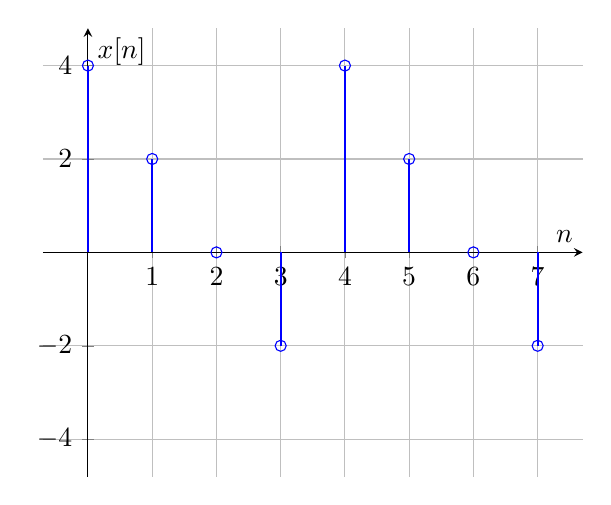
\begin{tikzpicture}
    \begin{axis}[
        axis lines=middle,
        xlabel={$n$},
        ylabel={$x[n]$},
        ymin=-4, ymax=4,
        xmin=0, xmax=7,
        xtick={1,2,3,4,5, 6, 7},
        ytick={-4, -2,0,2, 4},
        xticklabel style={/pgf/number format/.cd,fixed,precision=3},
        grid=both,
        enlargelimits=true,
    ]
        % Add vertical lines for each point in the stem plot
        \addplot [thick, blue] coordinates {(0, 0) (0, 4)};
        \addplot [thick, blue] coordinates {(1, 0) (1, 2)};
        \addplot [thick, blue] coordinates {(3, 0) (3, -2)};
        \addplot [thick, blue] coordinates {(4, 0) (4, 4)};
        \addplot [thick, blue] coordinates {(5, 0) (5, 2)};
        \addplot [thick, blue] coordinates {(7, 0) (7, -2)};
        
        % Plot markers at each stem point
        \addplot[mark=o, only marks, blue] coordinates {(0,4) (1,2) (2,0) (3,-2) (4,4) (5,2) (6,0) (7,-2)};
    \end{axis}
\end{tikzpicture}

\begin{enumerate}
    \item Compute the DTFS coefficients for this plot.
    \ans{
    \[X_k = \frac{1}{p}\sum_{n=0}^{p-1}x[n]e^{-i\frac{2\pi}{p}nk}\]
    
    \[X_0 = \frac{1}{4}\sum_{n=0}^{3}x[n]e^{-i\frac{\pi}{2}n(0)} = \frac{1}{4}(4 + 2 + 0 -2) = 1\]
    \[X_1 = \frac{1}{4}\sum_{n=0}^{3}x[n]e^{-i\frac{\pi}{2}n(1)} = \frac{1}{4}(4 + 2e^{-i\frac{\pi}{2}} + 0 - 2e^{-i\frac{3\pi}{2}}) = \frac{1}{4}(4 + 2(-i) + 0 - 2(i)) = 1 - i\]
    \[X_2 = \frac{1}{4}\sum_{n=0}^{3}x[n]e^{-i\frac{\pi}{2}n(2)} = \frac{1}{4}(4 + 2e^{-i\pi} + 0 - 2e^{-i3\pi}) = \frac{1}{4}(4 + 2(-1) + 0 - 2(-1)) = 1\]
    \[X_3 = \frac{1}{4}\sum_{n=0}^{3}x[n]e^{-i\frac{\pi}{2}n(3)} = \frac{1}{4}(4 + 2e^{-i\frac{3\pi}{2}} + 0 - 2e^{-i\frac{9\pi}{2}}) = \frac{1}{4}(4 + 2i - 0 - 2(-i)) = 1 + i\]
    }

    \vspace{1.5in}
    
    \item Which Fourier Basis coefficient corresponds to the highest frequency in our signal? What frequency does this coefficient correspond to in Hz?  
    % \textit{Hint: What is the highest frequency? Does that match with any basis vectors?}
    \ans{
        Among our DTFS coefficients, the one that corresponds to the highest frequency is the one with the highest value of $k$. Therefore, the Fourier Basis coefficient that corresponds to the highest frequency is $X_3$.

        The angular frequency for this coefficient is
        $$\omega = \frac{2\pi}{p}k = \frac{2\pi}{4}(3) = \frac{3\pi}{2}$$

        Converting to Hz gives us:
        $$f = \frac{\omega}{2\pi} = \frac{\frac{3\pi}{2}}{2\pi} = \frac{3}{4} = 0.75\text{Hz}$$

        Note that in discrete time, the above frequency would correspond to a signal with period $p = \frac{1}{f} = \frac{4}{3}$, which is not a valid period in discrete time. Thus, while it is the highest frequency we can capture for our original sound (which is a continuous signal before we digitally sample it), it would appear to be lower frequency $p = 4 \rightarrow f = 0.25\text{Hz}$ in the behavior of our discrete wave.
    }

    \vspace{0.5in}

    \item Now, we would like to reconstruct what the 16Animals hear by setting all Fourier coefficients above 0.5 Hz to zero (which is equivalent to being unable to hear the higher frequencies) and reconstructing our signal with the remaining coefficients. After reconstructing our signal in this way, what is the resulting signal $x'[n]$?:
    
    \textit{Hint: Try using the Synthesis Equation.}

    \ans{
        We can see that of our Fourier coefficients, the only one that exceeds the 0.5 Hz threshold is the highest frequency corresponding to $X_3$. Thus, using the results from our first part, we want to reconstruct the signal with
        \[X_0 = 1\]
        \[X_1 = 1 - i\]
        \[X_2 = 1\]
        \[X_3 = 0\]

        Plugging into the Synthesis Equation gives us:
        \begin{align*}
            x[n] &= \sum_{k=0}^{3} X_ke^{i\frac{2\pi}{4}nk} \\
            &= \sum_{k=0}^{3} X_ke^{i\frac{\pi}{2}nk} \\
            &= X_0e^{i\frac{\pi}{2}n(0)} + X_1e^{i\frac{\pi}{2}n(1)} + X_2e^{i\frac{\pi}{2}n(2)} + X_3e^{i\frac{\pi}{2}n(3)} \\
            &= (1)(1) + (1 - i)(i)^n + (1)(-1)^n + (0)
        \end{align*}

        Using this, we get:
        \begin{align*}
            &x'[0] = 1 + (1-i) + (1) = 3 - i \\
            &x'[1] = 1 + i-(-1) - 1 = 1 + i \\
            &x'[2] = 1 - 1 + i + (1) = 1 + i \\
            &x'[3] = 1 + (1-i)(-i) - 1 = -1-i
        \end{align*}

        Because our signal is periodic this means that:
        $$x'[n] = \begin{cases}
            3 - i, & n = 4p, p \in \mathbb{Z} \\
            1 + i, & n = 4p + 1, p \in \mathbb{Z} \\
            1 + i, & n = 4p + 2, p \in \mathbb{Z} \\
            -1 - i, & n = 4p + 4, p \in \mathbb{Z}
        \end{cases}$$

        As noted in the previous subpart, the signal component corresponding to $X_3$ is not perfectly sampled in the discrete wave provided. This results in the imaginary coefficients we have derived. If the signal were to be more finely sampled, known as the Nyquist sampling rate, then we might be able to reconstruct a more accurate model for our 16Animals' ears!
%     \begin{tikzpicture}
%     \begin{axis}[
%         axis lines=middle,
%         xlabel={$n$},
%         ylabel={$x[n]$},
%         ymin=-4, ymax=4,
%         xmin=0, xmax=0.5,
%         xtick={0.125,0.25,0.375,0.5},
%         ytick={-4, -2,0,2, 4},
%         xticklabel style={/pgf/number format/.cd,fixed,precision=3},
%         grid=both,
%         enlargelimits=true,
%     ]
%         % Add vertical lines for each point in the stem plot
%         \addplot [thick, blue] coordinates {(0.125, 0) (0.125, 3)};
%         \addplot [thick, blue] coordinates {(0.25, 0) (0.25, -1)};
%         \addplot [thick, blue] coordinates {(0.375, 0) (0.375, -1)};
%         \addplot [thick, blue] coordinates {(0.5, 0) (0.5, 3)};
        
%         % Plot markers at each stem point
%         \addplot[mark=o, only marks, blue] coordinates {(0.125,3) (0.25,-1) (0.375,-1) (0.5,3)};
%     \end{axis}
% \end{tikzpicture}

Note this is how actual compression works for audio data!
    }
    

    
    
\end{enumerate}
